\section{Inference} \label{sec:inference}

The \emph{inference} stage aims to generate personalized recommendations tailored to the user's query paper.
The inference process is designed to operate iteratively: Users can select one of the recommended papers as their new query paper, prompting the system to generate recommendations for the new query next.
This iterative approach forms a document sequence of queries and recommendations.
At any point in this sequence, users can adjust input parameters to better suit their preferences.

Before starting the inference process, preparatory setup steps are required to ensure the recommender system has access to all necessary data. These include assembling the base dataset, downloading pretrained language models or word embeddings, and precomputing the co-citation analysis, bibliographic coupling, and cosine similarity scores in the preceding training stage. A detailed setup guide is provided by the \emph{readnext} documentation\footnote{\url{https://joel-beck.github.io/readnext/setup}}.


\subsection{User Interface} \label{sec:user-interface}

\subsubsection*{Input Parameters}

To generate customized recommendations, the system requires three input parameters: a query paper identifier, feature weights for the Citation Recommender, and a language model for the Language Recommender.

The query paper serves as the anchor of the recommendation process, as all recommendations are tailored to this paper. Query papers might be ones the user is currently reading, recommended by a colleague, or found through a search engine. There are four options to specify the query paper:

\begin{itemize}
    \item The \emph{Semantic Scholar URL}, viewed in a web browser's address bar on the Semantic Scholar\footnote{\url{https://semanticscholar.org}} site.
    \item The \emph{Semantic Scholar ID}, a 40-character hexadecimal string appearing after the last forward slash in the Semantic Scholar URL.
    \item The \emph{arXiv URL}, observed in a web browser's address bar on the arXiv\footnote{\url{https://arxiv.org}} site.
    \item The \emph{arXiv ID}, a sequence starting with four numbers, followed by a dot, then another five numbers, found after the final forward slash in the arXiv URL.
\end{itemize}

Since all identifiers are rooted in the Semantic Scholar or arXiv databases, \emph{readnext} currently supports inference for query papers present on either of these platforms.

The second input encompasses feature weights for the Citation Recommender. These weights, defined by numerical values (either as floats or integers), apply to the publication date, paper citation count, author citation count, co-citation analysis score, and bibliographic coupling score.
They signify each feature's relative importance in the Citation Recommender.
As stated in \Cref{sec:citation-recommender}, the weights are normalized with the L1 norm, ensuring the results are not affected by the absolute magnitude of the weights.

The third input designates the language model for the Language Recommender, with choices like TF-IDF, BM25, Word2Vec, FastText, GloVe, BERT, SciBERT, and Longformer, detailed in \Cref{sec:language-recommender}. The selected language model is used to compute the semantic similarity between the abstracts of the query paper and all candidate papers.

While specifying the query paper is mandatory, both feature weights and the language model are optional. If feature weights or language model are not provided, the system defaults to the best performing parameters identified in the evaluation stage (\Cref{sec:evaluation}). However, users are encouraged to explore various configurations to find the one best suited to their needs.


\subsubsection*{Output Format}

The \emph{readnext} function returns a result object containing data about various components and intermediate results of the recommendation process. Above all, this object comprises four recommendation lists with 20 recommended papers each.
The recommendation lists are presented in a tabulated format, where rows represent individual recommendations.
The columns provide additional information such as the candidate paper's title, author, publication date, arXiv categories, and URLs for the corresponding Semantic Scholar and arXiv websites.

Depending on whether the Citation Recommender or the Language Recommender determines the recommendation list's ranking order, the table format differs slightly.

\begin{enumerate}
    \item If the table contains the Citation Recommender candidates or the \ac{L2C} hybrid model's recommendations,
          the ranking order is determined by the \emph{weighted points score} of the Citation Recommender. Candidates are sorted by their score in descending order, with the highest-scoring recommendation first.
    \item If the table contains the Language Recommender candidates or the \ac{C2L} hybrid model's recommendations,
          the ranking order is determined by the \emph{cosine similarity} between the abstract embedding of the query paper and the abstract embedding of the candidate paper. Candidates are sorted by their cosine similarity in descending order, placing the most similar candidate paper at the top.
\end{enumerate}


\subsection{Seen vs. Unseen Papers} \label{sec:seen-vs-unseen-papers}

Inference applies to papers included in the \emph{readnext} dataset (termed \emph{seen} papers) and those not included (termed \emph{unseen} papers). Although the user interface remains the same for both categories, their underlying inference methodologies differ markedly. The subsequent sections elucidate the inference procedure for both seen and unseen papers.

\subsubsection*{Input Validation}

Initially, the user input is parsed and validated through the \texttt{pydantic} library\footnote{\url{https://docs.pydantic.dev/latest/}}. Invalid inputs cause the program to exit early, displaying an informative error message.

The following checks are performed:

\begin{itemize}
    \item Exactly one of the four available query paper identifiers is provided.
    \item When specified, the Semantic Scholar ID is a 40-character hexadecimal string.
    \item When specified, the Semantic Scholar URL starts with \url{https://www.semanticscholar.org/paper/}.
    \item When specified, the arXiv ID starts with four digits followed by a dot followed by five more digits.
    \item When specified, the arXiv URL starts with \url{https://arxiv.org/abs/}.
    \item If feature weights are provided, they are non-negative numeric values.
    \item If a language model is provided, it belongs to one of the eight implemented models.
\end{itemize}

Post-validation, the query paper identifier is used to determine whether the query paper is included in the \emph{readnext} dataset, i.e., whether it is a seen or an unseen paper.


\subsubsection*{Inference for Seen Papers}

For seen query papers, the inference process is fast and efficient, as it mainly involves retrieving precomputed data from the training phase.
\Cref{fig:inference-seen} illustrates the inference process for seen query papers schematically.

\begin{figure}[ht!]
    \centering
    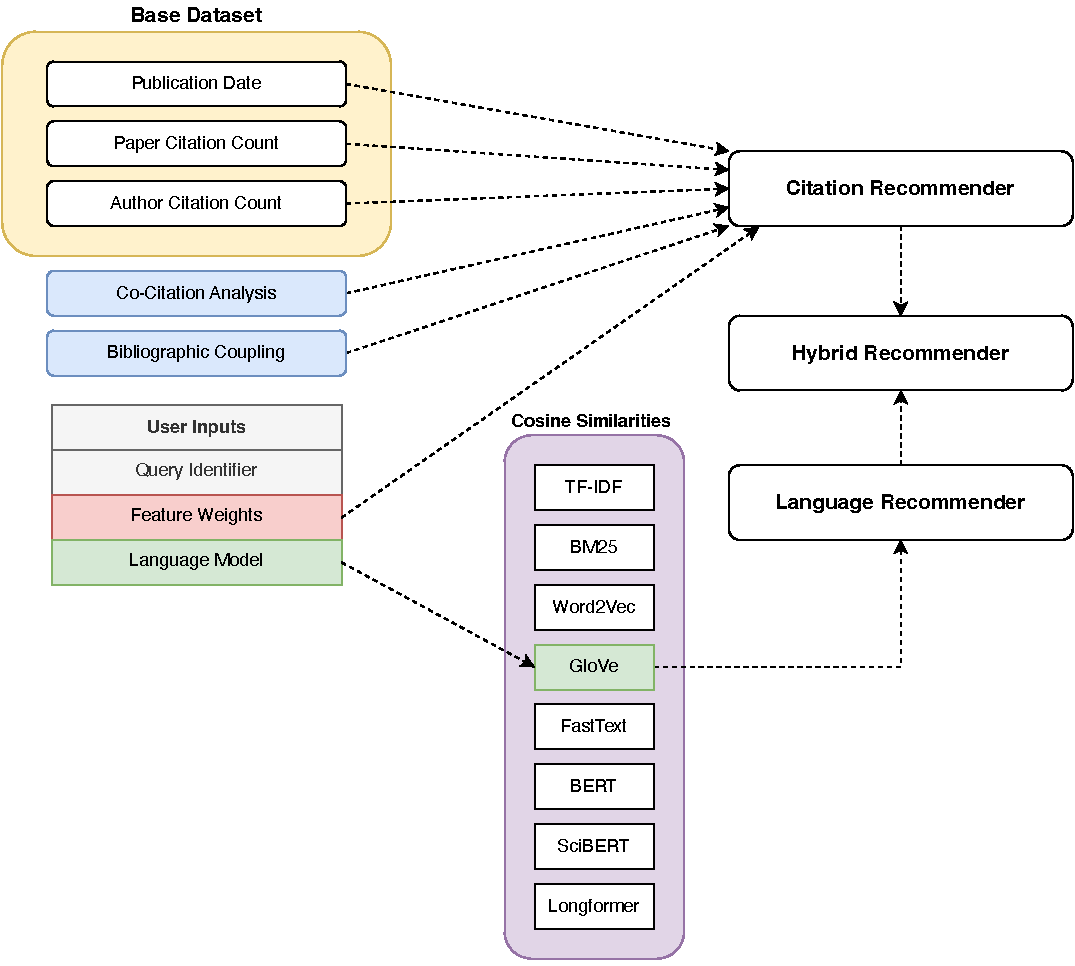
\includegraphics[width=\textwidth]{diagrams/inference_seen.pdf}
    \caption[Inference for Seen Papers]{Inference process for seen query papers.
        The Citation Recommender extracts global document features from the base dataset. Co-citation analysis scores and bibliographic coupling scores are retrieved from the precomputed data. The Language Recommender uses the precomputed cosine similarities. The Hybrid Recommender combines the candidate lists from the Citation Recommender and the Language Recommender to form the final recommendation ranking.}
    \label{fig:inference-seen}
\end{figure}

First, the query identifier provided by the user is converted into an internal document ID, which then serves as a key to access precomputed data from the data storage.
The lookup process is illustrated in \Cref{fig:inference-lookup} at the example of co-citation analysis scores.

\begin{figure}[ht!]
    \centering
    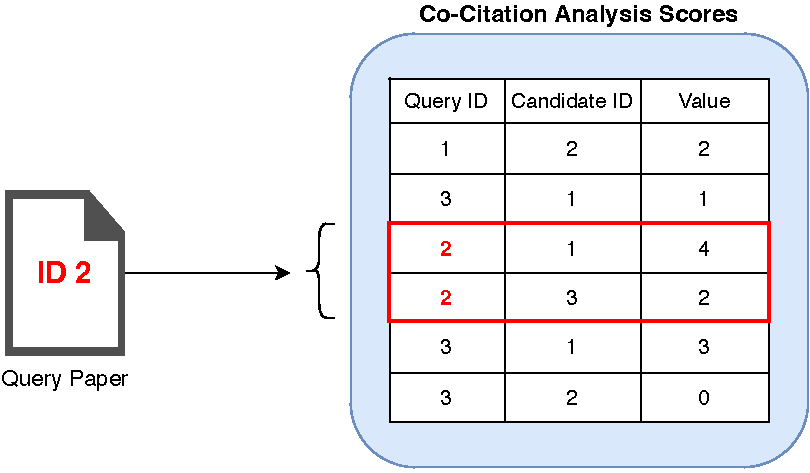
\includegraphics[width=0.7\textwidth]{diagrams/inference_lookup.pdf}
    \caption[Inference Lookup]{Lookup process for seen papers during inference using the example of co-citation analysis scores. The query paper's identifier is used to retrieve the relevant information from the precomputed scores. The scores are stored with their corresponding query and candidate paper IDs in long data format. Only the subset with a matching query paper ID is considered, as indicated by the red rectangle. The query-specific co-citation analysis scores are then ranked and converted to points.}
    \label{fig:inference-lookup}
\end{figure}

Second, the Citation Recommender uses the query paper's identifier to filter global document characteristics, precomputed co-citation analysis scores, and bibliographic coupling scores.
In this way, only the relevant information for the query paper is retrieved.
Next, point scores for each individual feature are computed as described in \Cref{sec:citation-recommender}. The individual points are weighted by the user-specified feature weights and summed to obtain the weighted points score. The top $n=20$ candidates with the highest score are returned as the Citation Recommender's candidate list.

Third, the Language Recommender filters the precomputed cosine similarities for the user-specified language model by the query paper's identifier.
The top $n=20$ candidates with the highest cosine similarity are returned as the Language Recommender's candidate list.

Finally, the Hybrid Recommender forms the final recommendation rankings from the candidate lists of the Citation Recommender and the Language Recommender.
For the \ac{C2L} hybrid model, the \emph{readnext} corpus is first reduced to the Citation Recommender's candidates.
The Language Recommender then sorts these papers by the cosine similarity between the query paper's abstract and the candidate papers' abstracts.
Conversely, for the \ac{L2C} hybrid model, the \emph{readnext} corpus is reduced to the Language Recommender's candidates and sorted by the weighted points score of the Citation Recommender.
The final and candidate rankings of both hybrid orderings are returned to the user.


\subsubsection*{Inference for Unseen Papers}

For unseen query papers, the inference process is more complex, as query-specific data cannot be retrieved from the training stage and must be computed on the fly. The inference process for unseen query papers is illustrated in \Cref{fig:inference-unseen}.

\begin{figure}[htb!]
    \centering
    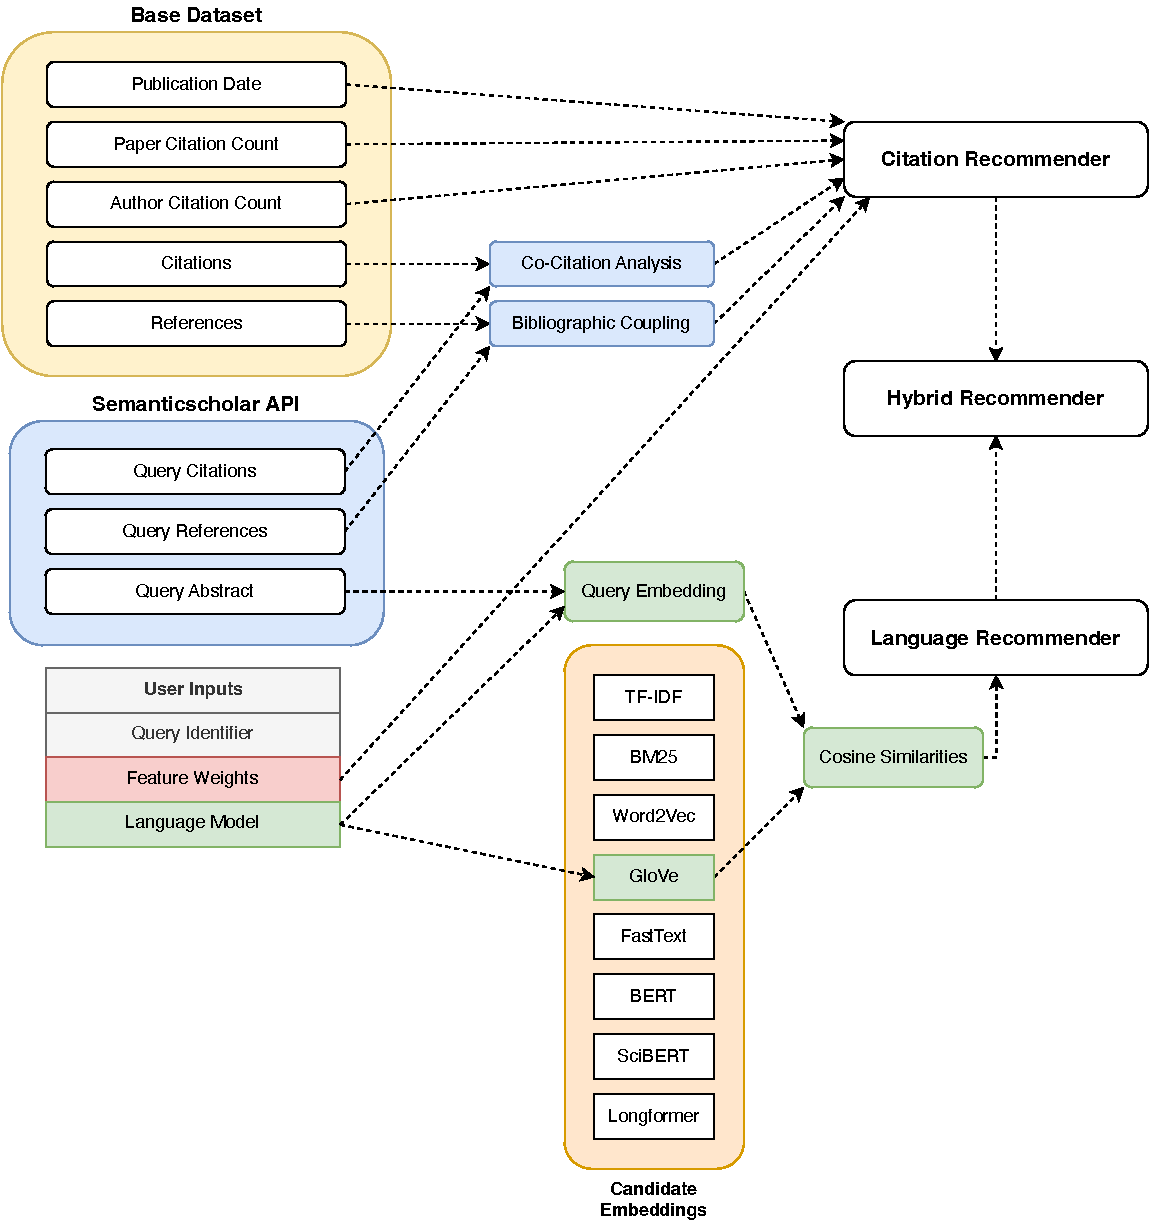
\includegraphics[width=\textwidth]{diagrams/inference_unseen.pdf}
    \caption[Inference for Unseen Papers]{Inference process for unseen query papers.
        Unlike the inference process for seen papers as detailed in \Cref{fig:inference-seen}, citations, references, and the abstract for the query paper are retrieved from the Semantic Scholar API.
        The Citation Recommender computes query-specific co-citation analysis scores and bibliographic coupling scores using global document characteristics and citation-based features for the candidates from the base dataset.
        The Language Recommender derives query-specific cosine similarities based on the query embedding and the stored candidate embeddings.
        Similar to the process for seen query papers, the Hybrid Recommender combines the candidate lists from both the Citation and Language Recommenders to generate the final recommendation ranking.}
    \label{fig:inference-unseen}
\end{figure}


First, the user-provided query identifier is converted to a valid Semantic Scholar URL or arXiv URL to fetch the query paper's metadata from the Semantic Scholar Academic Graph API, including the paper's title, authors, abstract, citations, and references.
Information regarding the query's global document characteristics — like the publication date, paper citation count, and author citation count — is not required. This is because the candidate rankings for these features do not depend on the query paper's characteristics.
As arXiv categories cannot be obtained from the Semantic Scholar API, label information is not available for unseen papers during inference.

Next, query-specific co-citation analysis and bibliographic coupling scores are computed by matching the query paper's citations and references with the corresponding lists of all candidates, as detailed in \Cref{fig:bibliographic_coupling_from_references}.
Similar to the inference process for seen papers, the Citation Recommender computes weighted point scores for all candidates and returns the top $n=20$ candidates as the Citation Recommender's candidates.

The Language recommender first tokenizes and embeds the query paper's abstract using the user-specified language model. The candidate embeddings can be retrieved from the precomputed data. Then, the query-specific cosine similarities between the query embedding and all candidate embeddings are computed. The subsequent steps mirror the inference process for seen papers, including the re-ranking performed by the Hybrid Recommender.


\subsection{Performance Considerations} \label{sec:performance-considerations}

Performance has been a key focus from the start of this project.
The value of a highly accurate recommender system diminishes if users face long waiting times to receive recommendations.
For instance, if a single inference run took 10 minutes, it would be impractical to use the system for exploratory purposes, such as comparing different model configurations.
In addition, searches with less personalized but faster systems could be refined several times in the same time frame, potentially yielding better results.

Although optimizing the computational complexity of both training and inference stages is desirable, the inference stage is more critical
This is because the training stage is performed only once, while the inference stage is executed each time a user requests recommendations. Therefore, in case of trade-offs between training and inference performance, the inference stage should be prioritized.

The main bottleneck for both training and inference runtime is the size of the training corpus, creating a trade-off between performance and coverage breadth.
On the one hand, a larger training corpus increases the coverage of the recommendations, minimizing the risk of excluding relevant papers from the corpus. On the other hand, as the corpus size increases, many operations during both training and inference become more complex and time-consuming.


\subsubsection*{Corpus Size \& Computational Complexity}

For seen query papers, the inference runtime is marginally, or not at all, affected by the number of candidate papers in the dataset. This is because the only change when doubling the corpus size is a lookup within a larger dataframe. Since lookups based on hash tables are run in constant time, the time complexity of this operation remains largely unaffected by the corpus size.

In contrast, inference runtime for unseen papers grows linearly with the corpus size. This is due to the need to compute query-specific co-citation analysis and bibliographic coupling scores as well as cosine similarities between the query paper and all candidate papers on-the-fly, with the number of candidate papers equaling the corpus size.
Thus, when the corpus size doubles, the number of pairwise scores that must be computed also doubles, resulting in a linear increase in runtime.

The most significant effect of the corpus size on the time complexity is during training.
Pairwise co-citation analysis scores, bibliographic coupling scores, and cosine similarities need to be computed for \emph{every} pair of papers in the \emph{readnext} dataset. Consequently, the time complexity of these operations grows quadratically with the corpus size.
In addition, memory and storage requirements also grow quadratically as the pairwise scores are saved to disk during training and loaded into memory during inference.


\subsubsection*{Strategies for Performance Optimization}

To tackle runtime issues, the base dataset is limited to the top $10,000$ most cited papers from the D3 dataset.
This corpus size strikes a balance between performance and coverage:
Inference time is reduced to less than two seconds for seen query papers and between 10 and 30 seconds for unseen query papers. In the latter case, the most time-consuming aspect is loading large pretrained language models or word embeddings into memory, a process that is difficult to optimize without resorting to smaller and less accurate models.

At the same time, the corpus size is large enough to cover a wide range of popular papers across various Computer Science disciplines.
The cut-off threshold for the $10,000$ most cited papers stands at $141$ citations; papers cited more often are included in the corpus.
This way, even lesser-known papers, especially those outside a researcher's field of expertise, can still be recommended.

To save on memory and storage, only the top $100$ candidate papers with the highest co-citation analysis, bibliographic coupling, and cosine similarity scores are stored for each query paper. \Cref{sec:citation-recommender} highlights how this limitation affects the Citation Recommender's scoring mechanism.
By storing a constant number of candidate papers for each query paper, the growth of memory and storage requirements is linear rather than quadratic.

When combined with a corpus size limit of $10,000$ papers, the storage requirements remain manageable.
For instance, the precomputed cosine similarities require 5 - 7 MB of storage space, depending on the language model. In comparison, increasing the corpus size to $100,000$ papers while storing \emph{all} pairwise scores would inflate these files to 0.5 - 0.7 GB. Further scaling to $1,000,000$ papers would necessitate 50 - 70 GB of storage space.
Thus, building a recommender system that scales to millions of papers requires a more complex storage architecture or a more sophisticated approach of handling the $O(n^2)$ complexity, like a preceding clustering step as proposed by Kanakia et al. \cite{KanakiaScalableHybrid2019}.
